\documentclass{beamer}
\usetheme{metropolis}
\title{Global Non-Determinism With Termination}
\date{\today}
\author{Pepijn Kokke}
\institute{University of Edinburgh}
\usepackage{microtype}
\usepackage{alphabeta}
\usepackage[greek,english]{babel}
\languageattribute{greek}{polutoniko}
\usepackage[dvipsnames,table]{xcolor}
\colorlet{tm}{Black}
\colorlet{ty}{Black}

\usepackage{fullpage}
\usepackage{amsmath, amscd, amsthm, amssymb, mathrsfs,amsfonts}
\usepackage{textcomp}
\usepackage{txfonts}
\usepackage{graphicx}

%%% TERM CALCULUS
\newcommand{\link}[2]{#1{\leftrightarrow}#2}
\newcommand{\wait}[1]{#1().}
\newcommand{\halt}[1]{#1[].0}
\newcommand{\send}[2]{#1[#2].}
\newcommand{\recv}[2]{#1(#2).}
\newcommand{\case}[3]{%
\toks0={#2#3}%
\edef\param{\the\toks0}%
\ifx\param\empty
  \ensuremath{\text{case} \; #1 \; \{\}}
\else
  \ensuremath{\text{case} \; #1 \; \{ #2 ; #3 \}}
\fi}
\newcommand{\inl}[1]{#1[\text{inl}].}
\newcommand{\inr}[1]{#1[\text{inr}].}
\newcommand{\expn}[2]{#1 \uparrow #2.}
\newcommand{\intl}[2]{#1 \downarrow #2.}
\newcommand{\cut}[1]{\nu #1.}

\def\parr{\ensuremath{\mathbin{\rotatebox[origin=c]{180}{\&}}}}
\def\with{\ensuremath{\mathbin{\text{\&}}}}
\def\plus{\ensuremath{\oplus}}
\def\tens{\ensuremath{\otimes}}
\def\limp{\ensuremath{\multimap}}
\def\one{\ensuremath{\mathbf{1}}}
\def\nil{\ensuremath{\mathbf{0}}}
\def\lequiv{\ensuremath{\multimapboth}}

\DeclareGraphicsRule{.ai}{pdf}{.ai}{}
\newcommand{\emoji}[2][1em]{\ensuremath{\vcenter{\hbox{\includegraphics[width=#1]{twemoji/assets/#2.ai}}}}}
\newcommand{\mary}[1][1em]{\emoji[#1]{1f469}}
\newcommand{\john}[1][1em]{\emoji[#1]{1f466}}
\newcommand{\cake}[1][1em]{\emoji[#1]{1f382}}
\newcommand{\plato}[1][1em]{\emoji[#1]{1f381}}
\newcommand{\nocake}[1][1em]{\emoji[#1]{1f64c}}
\newcommand{\money}[1][1em]{\emoji[#1]{1f4b0}}
\newcommand{\dollar}[1][1em]{\emoji[#1]{1f4b5}}
\newcommand{\ptis}[1][1em]{\emoji[#1]{1f3ea}}
\newcommand{\good}[1][1em]{\emoji[#1]{2714}}
\newcommand{\bad}[1][1em]{\emoji[#1]{2716}}

\newcommand{\tm}[2][]{%
\toks0={#1}%
\edef\param{\the\toks0}%
\ifx\param\empty
  \ensuremath{{\color{ty}#2}}%
\else
  \ensuremath{{\color{tm}#1}\colon{\color{ty}#2}}%
\fi}
\newcommand{\seq}[2][]{\ensuremath{{\color{tm}#1}\vdash{\color{ty}#2}}}
\newcommand{\subst}[3]{\ensuremath{#1 \{ #2 / #3 \}}}
\newcommand{\nod}[2][]{\ensuremath{{\star}_{#1}{#2}}}
\newcommand{\give}[2][]{\ensuremath{{ ? }_{#1}{#2}}}
\newcommand{\take}[2][]{\ensuremath{{ ! }_{#1}{#2}}}

\usepackage{bussproofs}
\def\fCenter{\ensuremath{\;\vdash\;}}
\newcommand{\NOM}[1]{\RightLabel{\textsc{#1}}}
\newcommand{\SYM}[1]{\RightLabel{\ensuremath{#1}}}
\EnableBpAbbreviations
\newenvironment{proofbox}[1][0.9]%
  {\gdef\scalefactor{#1} \leavevmode\hbox\bgroup}
  {\scalebox{\scalefactor}{\DisplayProof} \egroup}
\newenvironment{proofblock}[1][0.9]%
  {\gdef\scalefactor{#1}\begin{center}\proofSkipAmount \leavevmode}%
  {\scalebox{\scalefactor}{\DisplayProof}\proofSkipAmount \end{center} }

%%% Local Variables:
%%% TeX-master: "main"
%%% End:
\begin{document}

\maketitle

\begin{frame}{This is how I write \textpi-calculus things}
  \[\!
    \begin{aligned}
      P, Q ::=&\;\nu x.P        &&\text{create a new channel $x$}
      \\  \mid&\;x[y].P         &&\text{send a channel $y$ over $x$, then run P}
      \\  \mid&\;x(y).P         &&\text{receive a channel $y$ over $x$, then run P}
      \\  \mid&\;0              &&\text{halt}
      \\  \mid&\;\inl{x}P       &&\text{send a bit (inl) over $x$, then run P}
      \\  \mid&\;\inr{x}P       &&\text{send a bit (inr) over $x$, then run P}
      \\  \mid&\;\case{x}{P}{Q} &&\text{receive a bit over $x$, then run P or Q}
      \\  \mid&\;x[].P          &&\text{send a ping over $x$, then run P}
      \\  \mid&\;x().P          &&\text{receive a ping over $x$, then run P}
      \\  \mid&\;\case{x}{}{}   &&\text{loop}\]
  \end{aligned}
  
\end{frame}

\begin{frame}{Local choice}
  \centering
  \begin{tikzpicture}[sibling distance=3cm,level distance=3cm]
    \Tree
    [.{$P + Q$} \edge[->]; {$P$} \edge[->]; {$Q$} ]
  \end{tikzpicture}
\end{frame}

\begin{frame}{Non-determinism in the \textpi-calculus}
  \centering
  \begin{tikzpicture}[sibling distance=3cm,level distance=3cm]
    \Tree
    [.{$\nu x.(x(y).P \mid x(z).Q \mid x[a].x[b].0)$}
    \edge[->]; {$(\subst{P}{a}{y} \mid \subst{Q}{b}{z})$}
    \edge[->]; {$(\subst{P}{b}{y} \mid \subst{Q}{a}{z})$}
    ]
  \end{tikzpicture}
\end{frame}

\begin{frame}{``Local'' choice in the \textpi-calculus}
  \centering
  \only<1>{%
    \begin{tikzpicture}[sibling distance=3cm,level distance=3cm]
      \Tree
      [.{$\nu x.(x().P \mid x().Q \mid x[].0)$}
      \edge[->]; {$\nu x.(P \mid x().Q)$}
      \edge[->]; {$\nu x.(x().P \mid Q)$}
      ]
    \end{tikzpicture}
  }
  \only<2>{%
    \begin{tikzpicture}[sibling distance=3cm,level distance=3cm]
      \Tree
      [.{$\nu x.(\case{x}{P}{0} \mid \case{x}{Q}{0} \mid \inl{x}\inr{x}{0})$}
      \edge[->]; {$P$}
      \edge[->]; {$Q$}
      ]
    \end{tikzpicture}
  }
\end{frame}

\begin{frame}{Non-determinism in the \textpi-calculus using local choice}
  \centering
  \begin{tikzpicture}[sibling distance=3cm,level distance=3cm]
    \Tree
    [.{$(\subst{P}{a}{y} \mid \subst{Q}{b}{z}) + (\subst{P}{b}{y} \mid \subst{Q}{a}{z})$}
    \edge[->]; {$(\subst{P}{a}{y} \mid \subst{Q}{b}{z})$}
    \edge[->]; {$(\subst{P}{b}{y} \mid \subst{Q}{a}{z})$}
    ]
  \end{tikzpicture}
\end{frame}

\begin{frame}{Local choice is not modular}
  \only<1>{%
    If we extend...
    \[
      \nu x.(x(y).P \mid x(z).Q \mid x[a].x[b].0)
    \]
    ...to...
    \[
      \nu x.(x(y).P \mid x(z).Q \mid x(w).R \mid x[a].x[b].x[c].0)
    \]
  }
  \only<2>{%
    Then we must extend...
    \[
      (\subst{P}{a}{y} \mid \subst{Q}{b}{z}) + (\subst{P}{b}{y} \mid \subst{Q}{a}{z})
    \]
    ...to...
    \[\!
      \begin{array}{cc}
        (\subst{P}{a}{y} \mid \subst{Q}{b}{z} \mid \subst{R}{c}{w}) &+ \\
        (\subst{P}{b}{y} \mid \subst{Q}{a}{z} \mid \subst{R}{c}{w}) &+ \\
        (\subst{P}{a}{y} \mid \subst{Q}{c}{z} \mid \subst{R}{b}{w}) &+ \\
        (\subst{P}{b}{y} \mid \subst{Q}{c}{z} \mid \subst{R}{a}{w}) &+ \\
        (\subst{P}{c}{y} \mid \subst{Q}{a}{z} \mid \subst{R}{b}{w}) &+ \\
        (\subst{P}{c}{y} \mid \subst{Q}{b}{z} \mid \subst{R}{a}{w})
      \end{array}
    \]
  }
\end{frame}


\end{document}